\chapter{Analysing C++ Code}\todo{proper name}
\label{chap:AnalysingCPP}

To retrieve information about elements declared in \myProperName{C++} header files, a shared library called \myProperNameImp{CPPAnalyzer} was written in \myProperName{C++}. The library uses \myProperNameImp{libclang} for parsing \myProperName{C++} files and accessing AST information. Internally a reduced syntax tree is built and exported as the data interchange format \myProperName{JSON (JavaScript Object Notation)}.

The library exposes its functionality in form of a \myProperName{C} interface. It uses features from the new \myProperName{C++} standard \myProperName{C++11} (including the \mySCName{auto} keyword, but more importantly the regular expression functionality of the standard library). \myProperName{CPPAnalyzer} is currently built using \myProperName{Visual Studio 2010} on \myProperName{Windows 7} 64-bit. Other operating systems or compilers have not been tested, but should be supported with minor modifications.

\section{\myProperName{libclang}}

As explained in \myRefSection{sec:Clang}, \myProperName{libclang} is a \myProperName{C} interface to \myProperName{Clang} that can be used for accessing \myProperName{Clang}'s parsing functionality and internal abstract syntax tree (AST).

The two most important data structures \myProperName{libclang} provides, are \mySCName{CXCursor} and \mySCName{CXType}.
\\\mySCNameImp{CXCursor} represents a single node in the AST. It holds an enum constant (named \mySCName{kind}) that identifies the kind of the AST node - whether it is a namespace, function declaration, class declaration, etc. The \myProperName{C} struct \mySCName{CXCursor} internally stores information about the corresponding \myProperName{Clang} data in an array of \mySCName{void} pointers.
\\\mySCNameImp{CXType} represents a \myProperName{C++} type. It holds the kind of the type, for example if it is a pointer, reference, builtin type (like \mySCName{int} or \mySCName{float}), record (\mySCName{class} or \mySCName{struct}), etc. Just like \mySCName{CXCursor}, it also stores information about the \myProperName{Clang} type representation.

More information about cursors and types can be retrieved using the functions \myProperName{libclang} provides.
\\If the user, for instance, wants to know if a member function is declared as \mySCName{virtual}, he will call \mySCName{clang\_isCXXMethodVirtual} and pass a cursor that represents a member function (e.g. with the kind \mySCName{CXCursor\_CXXMethod}) to it. \mySCName{clang\_getCursorType}, as another example, will return the type of a variable or parameter declaration as a \mySCName{CXType}.

\mySCName{clang\_parseTranslationUnit} is the starting point for parsing \myProperName{C++} files. The function \myInlineQuote{accepts a set of command-line arguments so that the compilation can be configured in the same way that the compiler is configured on the command line}\footnote{\citep{ClangAPIDoc}}. These options commonly contain the path to the \myProperName{C++} file that is to be parsed. The function returns a translation unit, which holds all the AST information and from which the root cursor of the AST can be retrieved. While parsing, \myProperName{Clang} produces diagnostic information, for example when mal-formed \myProperName{C++} code was provided or other errors occur. \myProperName{libclang} provides functionality to access these diagnostics.

To traverse the abstract syntax tree recursively, \mySCName{clang\_visitChildren} is used. The function takes 3 arguments: the cursor to be visited; a function pointer, which serves as a callback that is called for every visited child; and a \mySCName{void} pointer for user data. The callback function will be called from \myProperName{Clang}, passing the visited cursor, its parent and the user data as parameters. This function is used to inspect and analyse the child cursor that it receives. The return value of the callback function tells \myProperName{Clang}, whether it should go on recursively with the first child of the passed child cursor, go on with the next sibling or if it should end the traversal of the AST at this point.

\myProperName{libclang} provides more than 50 functions that deal with AST inspection - far too many, to be covered in this thesis. A complete overview is given at the \myProperName{libclang} doxygen documentation\footnote{\myProperName{libclang} reference: \url{http://clang.llvm.org/doxygen/group\_\_CINDEX.html}}.

\subsection{Extending \myProperName{libclang}}

\myProperName{libclang} does not expose all of the functionality \myProperName{Clang} provides. Functionality missing in \myProperName{libclang} is added on a per-need basis. 

During this thesis it became clear that I need to extend \myProperName{libclang} to expose AST information about \myProperName{C++} templates. It seems, such information was not needed by other \myProperName{libclang} users. The changes I made to the \myProperName{libclang} source code base will hopefully make its way back into the official \myProperName{Clang} repository.

Most of the functions added to \myProperName{libclang} simply forward \myProperName{Clang}'s internals. Therefore the \myProperName{Clang} data needs to be retrieved from the \mySCName{CXCursor}s and \mySCName{CXType}s. Even though the functionality is often just forwarded, the \myProperName{Clang} code base needed to be understood and used in an appropriate  manner.

When turning \myProperName{Clang} types into \mySCName{CXType}s, certain \myProperName{C++} types were not exposed. \myProperName{libclang} was altered to support template type parameter types (\mySCName{TemplateTypeParm}), template specialization types and elaborated types (types that are sugared with a type keyword like \mySCName{class} and/or a prefixed namespace identifier). \myRefListing{lst:ClangNewTypes} shows examples of such types.

\SingleSpacing
\begin{lstlisting}[language=C++, caption=Examples of types now supported by \myProperName{libclang}, label=lst:ClangNewTypes]
template<class T>
class TemplatedClass
{
	// NEW: type of kind TemplateTypeParm
	T member; 
};

// NEW: type of kind TemplateSpecialization
TemplatedClass<int> tempSpecInstance; 

namespace SomeNamespace
{	
	class NormalClass{};
	
	// OLD: type of kind Record
	NormalClass instance;
	
	// NEW: type of kind Elaborated
	class NormalClass elaboratedInstance1;
}

// NEW: type of kind Elaborated
SomeNamespace::NormalClass elaboratedInstance2; 
\end{lstlisting}
\OnehalfSpacing

\myProperName{libclang} already exposed template parameters as \mySCName{CXCursor}s, when visiting the children of a class, struct or function cursor. Helper functions for accessing the template parameters directly from cursor, were added to \myProperName{libclang}:

\vspace{-10pt}
\begin{itemize}\addtolength{\itemsep}{-0.5\baselineskip}
\item \mySCName{unsigned clang\_getTemplateNumParameters(CXCursor C);}
\item \mySCName{CXCursor clang\_getTemplateParameter(CXCursor C, unsigned Index);}
\end{itemize}
\vspace{-10pt}

\myProperName{libclang} did not expose any information about template arguments. Template arguments are the actual types used for template parameters, when instantiating a template. Functions for retrieving template arguments and their values (as type, integral, etc.) were added:

\vspace{-10pt}
\begin{itemize}\addtolength{\itemsep}{-0.5\baselineskip}
\item Added cursor kinds\begin{itemize}\addtolength{\itemsep}{-0.5\baselineskip}
	\item \mySCName{CXCursor\_TemplateNullArgument}
	\item \mySCName{CXCursor\_TemplateTypeArgument}
	\item \mySCName{CXCursor\_TemplateDeclarationArgument}
	\item \mySCName{CXCursor\_TemplateIntegralArgument}
	\item \mySCName{CXCursor\_TemplateTemplateArgument}
	\item \mySCName{CXCursor\_TemplateTemplateExpansionArgument}
	\item \mySCName{CXCursor\_TemplateExpressionArgument}
	\item \mySCName{CXCursor\_TemplatePackArgument}
	\end{itemize}
\item Added functions\begin{itemize}\addtolength{\itemsep}{-0.5\baselineskip}
	\item \mySCName{unsigned clang\_isTemplateArgument(CXCursor C);}
	\item \mySCName{unsigned clang\_getTemplateSpecializationNumArguments(CXCursor C);}
	\item \mySCName{CXCursor clang\_getTemplateSpecializationArgument(CXCursor C, \\unsigned Index);}
	\item \mySCName{CXType clang\_getTemplateArgumentValueAsType(CXCursor C);}
	\item \mySCName{long long clang\_getTemplateArgumentValueAsIntegral(CXCursor C);}
	\item \mySCName{CXCursor clang\_getTemplateArgumentValueAsDeclaration(CXCursor C);}
	\item \mySCName{CXCursor clang\_getTemplateArgumentValueAsTemplate(CXCursor C);}
	\item \mySCName{CXCursor clang\_getTemplateArgumentValueAsExpression(CXCursor C);}
	\end{itemize}
\end{itemize}
\vspace{-10pt}

Also a utility function for retrieving the access (\mySCName{private}, \mySCName{protected} or \mySCName{public}) of a \myProperName{C++} member field/function/subclass was added:

\vspace{-10pt}
\begin{itemize}\addtolength{\itemsep}{-0.5\baselineskip}
\item \mySCName{CX\_CXXAccessSpecifier clang\_getCXXMemberAccessSpecifier(CXCursor);}
\end{itemize}
\vspace{-10pt}

Before, the \myProperName{C++} access specifier cursors (e.g. \mySCName{public:}) had to be tracked manually during analysis of classes. The members' access was set according to the last found access specifier.

\section{Building a Simplified AST}

\myProperName{libclang} provides an AST that contains a lot of information, which is not needed for language binding purposes. Thus, a simplified abstract syntax tree is created that holds all necessary information in form of a tree structure.

The creation of the simplified AST is processed inside the \mySCNameImp{Clang\_AST} class and happens roughly in the following steps:

\begin{enumerate}\addtolength{\itemsep}{-0.5\baselineskip}
\item Create an intermediate AST that closely resembles the cursor tree that \myProperName{Clang} generates, filtering based on the cursor kind
\item Filter the intermediate tree based on user-given filters for file- and symbol name
\item For the nodes that are left, create data structures (of type \mySCName{ASTObject}) that hold information about the AST node and retrieve its properties using the \myProperName{libclang} API. Create data structures that hold type information (\mySCName{ASTType}) along the way.
\item Connect the \mySCName{ASTObject}s to form the final simplified AST 
\end{enumerate}

\subsection{The Intermediate AST}

In \myProperName{C++}, the same object (for example a function or class) can be declared multiple times, but only defined once. This property is sometimes used to eliminate unnecessary includes or avoid cyclic file dependencies, by providing forward declarations.\\
In \myProperName{Clang}, every declaration is a single AST node. This information is mostly unnecessary for glue code generation, thus AST nodes that represent the same \myProperName{C++} entity are combined in the intermediate AST. \myProperName{libclang} provides this functionality with the concept of a \textbf{canonical cursor} - a single cursor that represents all declarations of the underlying entity.

The intermediate tree is built using instances of \mySCNameImp{Clang\_AST\_CXTreeNode}, which can be seen in \myRefFigure{fig:CXTreeNode}. 

\begin{figure}[h] % h = here
	\centering
		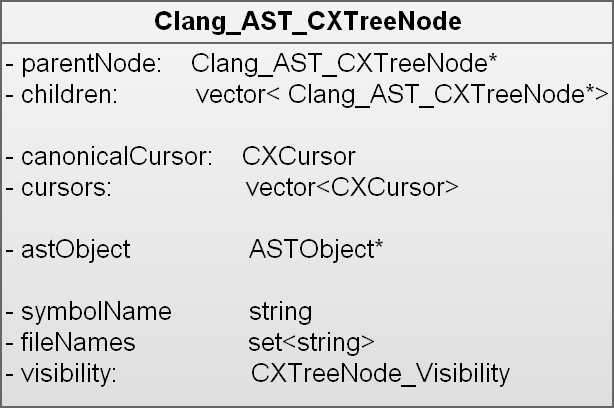
\includegraphics[scale=0.3]{Images/CXTreeNode.png}
	\caption{Members of an intermediate tree node}
	\label{fig:CXTreeNode}
\end{figure}

Every node holds a pointer to its parent and all of its children, resulting in a tree structure that can be traversed in both directions. 
The \mySCName{Clang\_AST} holds a reference to the root tree node and a map that links canonical cursors to intermediate tree nodes (for faster access).

After the translation unit has been parsed using \mySCName{clang\_parseTranslationUnit}, all the children of the translation unit cursor are visited with the help of \linebreak\mySCName{clang\_visitChildren}. Every visited child cursor is checked, whether an intermediate tree node has already been created for it - based on the child's canonical cursor. If so, the tree node is retrieved, the visited cursor added to its list of cursors and the children are visited. Visiting the children for an already existing tree node is necessary, as the the new found cursor may contain more children. This happens, for example, when the new found cursor represents a class definition.\\
If no tree node is existing for the canonical cursor, then, depending on the cursor's kind, a new tree node is created, inserted into the tree and added to the map that links canonical cursors and tree nodes. A lot of AST nodes are not needed for language binding. Thus, the first filtering happens at this stage and tree nodes for the intermediate AST are only created for the following \myProperName{C++} entities:\\global and static variables, \mySCName{union}, \mySCName{typedef}, \mySCName{struct}, \mySCName{namespace}, \mySCName{class} (including templated classes, partial specializations and explicit/implicit specializations), (templated) functions, function parameters, member functions, constructors, destructors, fields (data members), \mySCName{enum}, enum constants, template parameters, template arguments and linkage specifiers (e.g. \mySCName{extern "C"}).\\
From this list, it is obvious, that the intermediate AST will only have details up to function-level. Source code inside functions is not considered. 

\subsection{User-Based Filtering}

Parsing code that includes heavy libraries, like the \myProperName{C++} standard library or \myProperName{Boost}\footnote{\myProperName{Boost}: \url{http://www.boost.org/}}, results in a massive AST containing classes and other entities that the end-user might not want to create language bindings for and can as such be considered noise. With the help of different user-provided filters, the amount of nodes in the AST can be vastly reduced. 

At the time of creation, every tree node has been marked as \textbf{not visible}. Only nodes that are marked \textbf{visible} or \textbf{referenced} will appear in the final simplified AST. Referenced nodes are AST nodes that were initially filtered out, but are used by other nodes as a parent or for type information. As such, these nodes are an integral part of a consistent AST, where every node is a) supposed to be reachable while traversing the tree and b) expected to exist in the final tree when being referenced by another node.

In the filtering step every node of the intermediate tree is checked.

First the filename is checked with the help of a user-given regular expression. As a tree node may combine multiple cursors, the filenames of all these cursors are retrieved and matched against the regular expression. If none succeeds, the node and all its children are considered \textit{not visible}.

The second filter matches the complete symbol name of a node (mangled with all parent names added upfront) against a regular expression. Some nodes, like linkage specifiers, are not checked, as they do not have a name. If the symbol name check fails, then - depending on the kind of node (for example \mySCName{namespace}) - the algorithm still checks the visibility of the children as the symbol name filter may apply to those.

The third filter checks the member access of a node - whether it is \mySCName{private}, \mySCName{protected} or \mySCName{public}. For language binding, non-\mySCName{public} members are not needed as they can not be referenced by glue code.

If the tree node passes all three filters, it will be marked as \textit{visible}. As explained in more detail in the next section, an \mySCName{ASTObject} - a node of the final AST - will be created and stored in the intermediate tree node. Also, all parent nodes (that are still marked as \textit{not visible}) will be marked as \textit{referenced} and consequently appear in the final AST.

Depending on the kind of node, the visibility of the children is checked recursively.

\subsection{The Final AST}

The final simplified AST is a tree structure made of classes that inherit from
\mySCNameImp{ASTObject}. A single class exists for every kind of AST node. Only linkage specifiers will not appear in the final AST. The descendants of \mySCName{ASTObject} hold information according to their kind. \mySCName{ASTObject\_Function}, for example, holds information about its return type and parameters. \myProperName{Clang} treats static data members as variable declarations. The simplified AST will treat them as instances of \mySCName{ASTObject\_Field} that have the \mySCName{static} member set to \mySCName{true}.\\
An overview over the existing subclasses of \mySCName{ASTObject} can be found in \myRefFigure{fig:ASTObjectUML}.\\

\begin{figure}[h!] % h = here
	\centering
		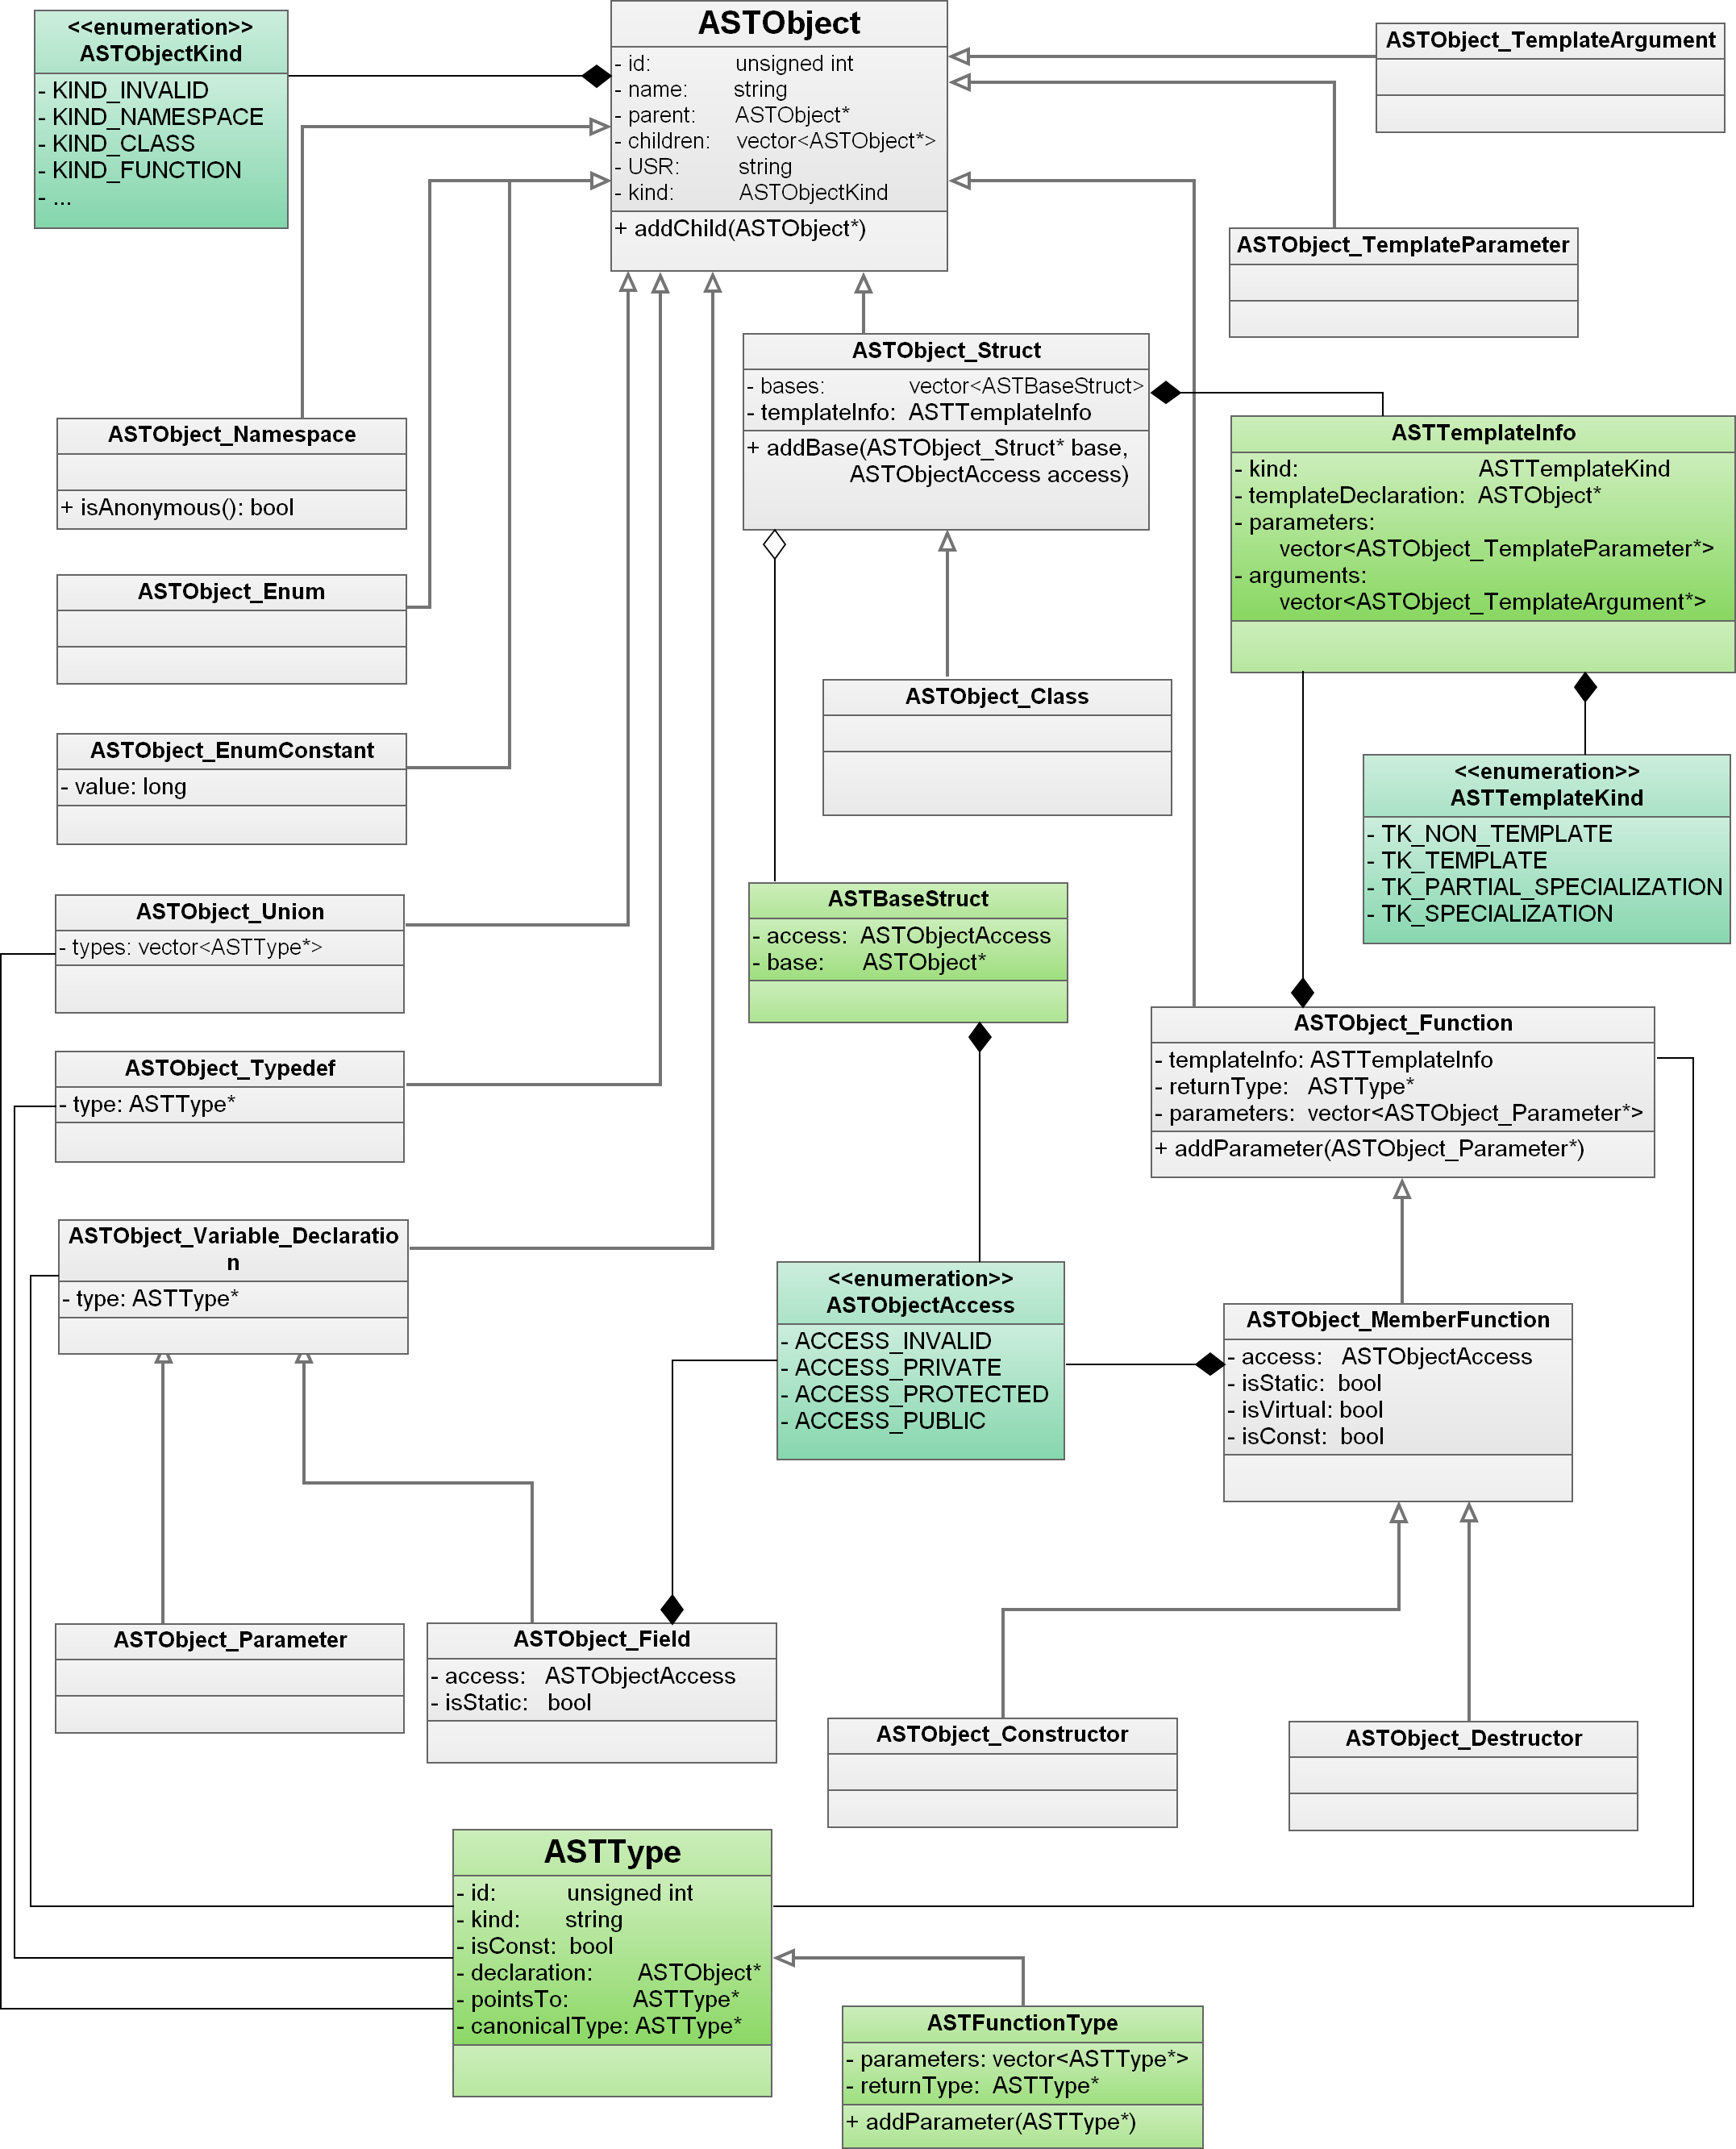
\includegraphics[scale=0.2]{Images/ASTObjectUML.png}
	\caption{\mySCName{ASTObject} classes and \mySCName{ASTType} (not all associations shown)}
	\label{fig:ASTObjectUML}
\end{figure}

\newpage
Just like \mySCName{Clang\_AST\_CXTreeNode}s, the \mySCName{ASTObject}s store a pointer to their parent and children and hence form a tree that can be traversed in both directions.

\mySCName{ASTObject}s are created whenever an intermediate tree node is marked \textit{visible} or \textit{referenced}.

When creating the specific \mySCName{ASTObject}s, the information belonging to the nodes is retrieved using the functions provided by \myProperName{libclang}. This includes template information, base class information, member access, function parameters, type information and much more.

Type information - exposed by \myProperName{libclang} as \mySCName{CXType} - will be saved as instances of \mySCNameImp{ASTType}. Apart from the kind of type (\mySCName{int}, \mySCName{float}, pointer, reference, record, \mySCName{typedef}, etc.), \mySCName{ASTType} also stores information about the declaration \mySCName{ASTObject} it refers to (for record and \mySCName{typedef} types), the pointee-type (for pointer and reference types) and whether the type is declared as \mySCName{const}. It also stores a pointer to the canonical type, which is the same type in its completely desugared form (all \mySCName{typedef}s removed). \mySCName{ASTFunctionType} stores the return type as well as the types of all parameters of a function type.

While creating \mySCName{ASTObject}s and \mySCName{ASTType}s, other \mySCName{ASTObject}s and \mySCName{ASTType}s will be referenced. In case the belonging intermediate tree nodes are marked as \textit{not visible}, these nodes and all their parent nodes have to be marked as \textit{referenced} and their \mySCName{ASTObject}s created, so they can be referenced by the other AST nodes of the final tree. In some cases, for example for implicit template specializations, the intermediate tree nodes do not exist yet. They have to be created and inserted before creating the corresponding \mySCName{ASTObject}.

In the final step, the intermediate tree is traversed from top to bottom and the existing \mySCName{ASTObject}s are connected with the next existing \mySCName{ASTObject} up in the parent chain. Remember: for some nodes, like linkage specifiers, no \mySCName{ASTObject}s have been created. These nodes will not appear in the final \mySCName{ASTObject} tree.

The final simplified AST is now finished and ready for further use in the application. From this point on, \myProperName{libclang} is not used anymore.

There are AST nodes and types that are not exposed by \myProperName{libclang}. If such a node or type is detected, a warning message is stored in a logger that belongs to the \mySCName{Clang\_AST}.

\newpage
\subsection{From Source Code to Simplified AST}

This section shows a small example demonstrating the algorithm described above.

\SingleSpacing
\begin{lstlisting}[language=C++, caption=Example input code for \myProperName{CPPAnalyzer}]
namespace SomeNamespace
{
	class SomeClass;
	
	class SomeClass
	{
		int member;
	};
	
	int aFunction(float param)
	{
		float res = param * 3;
		return res;
	}
}

extern "C"
{
	void dontFilter(SomeClass pInstance){};
}
\end{lstlisting}
\OnehalfSpacing

\vspace{15pt}
\begin{figure}[h] % h = here
	\centering
		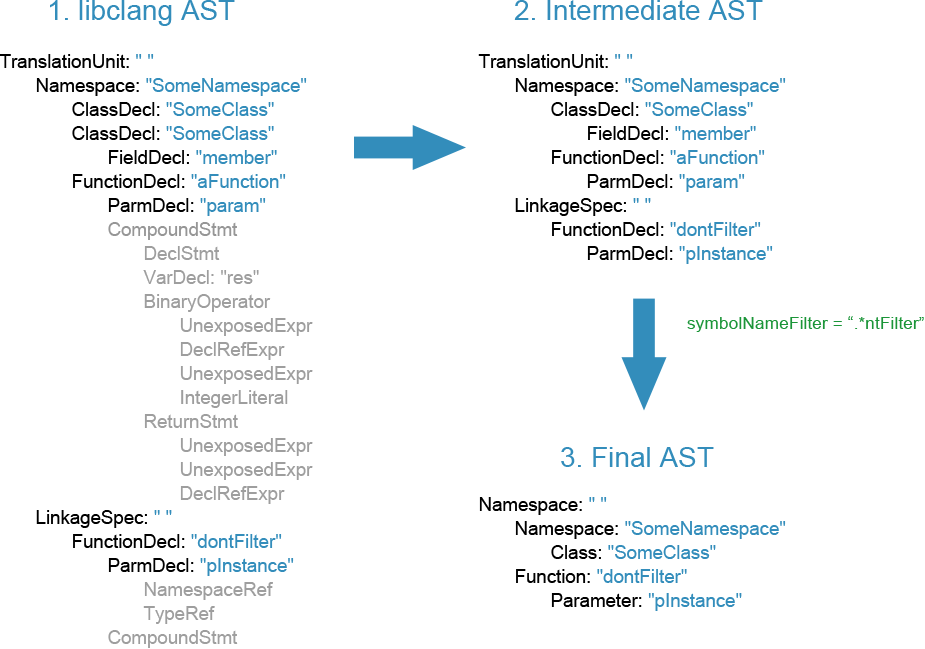
\includegraphics[scale=0.45]{Images/TreeExample.png}
	\caption{Comparison of generated ASTs}
	\label{fig:TreeExample}
\end{figure}


As can be seen in \myRefFigure{fig:TreeExample}, the AST \myProperName{Clang} produces contains a lot of unnecessary information. The intermediate AST removes many kinds of cursors and combines multiple declarations for the same entity. The final AST is filtered based on user-given options. In the example the function \mySCName{dontFilter} is the only node that was marked \textit{visible}, because it is the only node that matched the symbol name filter (\mySCString{.*ntFilter}). \mySCName{pInstance} is referenced as a parameter of \mySCName{dontFilter}. \mySCName{SomeClass} is referenced by the \mySCName{ASTType} used in \mySCName{pInstance}. Thus \mySCName{SomeClass} and its parent \mySCName{SomeNamespace} are marked as \textit{referenced} and as such are visible in the final tree. Note that the children of \mySCName{SomeClass} are not visible.

\section{Exporting the AST to \myProperName{JSON}}
\label{sec:ExportJSON}

As the AST will be used from within another application, it needs to be serialized into a string for passing the data across application borders. As will be shown in \myRefChapter{chap:GUIApplication}, the GUI application is heavily based on \myProperName{JavaScript}.\\
Hence, it is only logical that the AST is serialized into a string conforming the \myProperNameImp{JavaScript Object Notation (JSON)}. \myProperName{JSON}  is a lightweight data-interchange format, based on a subset of the \myProperName{JavaScript} programming language. The format is easy for humans to read and write, but also for machines to parse and generate.\footnote{\citep{JSONHP}}

The class \mySCNameImp{JSON\_Converter} was written to perform this task given an instance of \linebreak\mySCName{Clang\_AST}.

The first version of the converter was written without any additional libraries and handled the concatenation of the \myProperName{JSON} string itself. This was cumbersome and lead to code that was hard to maintain and error-prone. The \myProperName{JSON}-producing code was rewritten to use the library \myProperNameImp{JsonCpp}\footnote{\myProperName{JsonCpp}: \url{http://jsoncpp.sourceforge.net/}}.

The export is straight forward and the tree structure can basically be exported as is. \mySCName{ASTType}s and \mySCName{ASTObject}s, as well as their members, need to be converted into \myProperName{JSON} objects. All \mySCName{ASTType}s and \mySCName{ASTObject}s contain a unique id, which is used for cross-referencing. In both cases, the ids are numbers starting at 1.

The list of \mySCName{ASTType}s is converted first, followed by the tree of \mySCName{ASTObject}s. Logger messages produced during AST creation are also exported. The produced \myProperName{JSON} does not necessarily follow that order, as members of \myProperName{JSON} objects are sorted alphabetically in \myProperName{JsonCpp}.

\SingleSpacing
\begin{lstlisting}[language=C++, caption=Example AST for \myProperName{JSON} conversion]
class SomeClass
{
	public:
		int member;
};

SomeClass instance;
\end{lstlisting}
\OnehalfSpacing

\SingleSpacing
\begin{lstlisting}[language=JavaScript, caption=AST converted to \myProperName{JSON} (reduced example), label=listing:JSON]
{
   "AST" : {
      "rootASTObject" : {
         "id" : 1,
         "kind" : "Namespace",
         "name" : ""
         "children" : [{
               "id" : 2,
               "name" : "SomeClass",
               "kind" : "Class",
               "children" : [{
                     "id" : 3,
                     "name" : "member",
                     "kind" : "Field",
                     "access" : "public",
                     "type" : 1
                  }],
            },{
               "id" : 4,
               "name" : "instance",
               "kind" : "VariableDeclaration",
               "type" : 2
            }],
      }, // end of "rootASTObject"
      "types" : [{
            "id" : 1,
            "kind" : "Int"
            "isConst" : false,
         },{
            "id" : 2,
            "kind" : "Record"		 
            "declaration" : 2,
            "isConst" : false,
         }] // end of "types"
   }, // end of "AST"
   "log" : {
      "Clang" : [{
            "message" : "warning: 'linker' input unused when 
                '-fsyntax-only' is present", "type" : "Warning" }]
   }
}
\end{lstlisting}
\OnehalfSpacing

As can be seen in \myRefListing{listing:JSON}, the field \mySCName{member} references the type with the id 1, while the type 2 used by \mySCName{instance} references the AST node with the id 2, which is \mySCName{SomeClass}.

\newpage
\section{Calling the \myProperName{CPPAnalyzer}}
\label{sec:CallingCPPAnalyzer}

The \myProperName{CPPAnalyzer} shared library provides a \myProperName{C} interface through which it can be called.

\SingleSpacing
\begin{lstlisting}[language=C++, caption=\myProperName{CPPAnalyzer} \myProperName{C} API]
struct ParserInfo
{
	char* astTreeJSON;
};

extern "C"
{
	/** Frees the given parser info */
	CPPANALYZER_API void free_ParserInfo(ParserInfo* pi);

	/** Parses a header file and returns the filtered AST as JSON
	 *
	 * \param   argc           Number of arguments passed to Clang
	 * \param   argv           Command-line arguments passed to Clang
	 * \param   filterFile     Filename used for filtering
	 * \param   filterName     String used for symbol name filtering
	 * \param   filterAccess   Access filter
	 *
	 * \return   Parser information with AST in JSON
	 */
	CPPANALYZER_API ParserInfo* parse_header(int argc, char *argv[], 
				const char* filterFile, const char* filterName, 
				int filterAccess);
}
\end{lstlisting}
\OnehalfSpacing

The function \mySCName{parse\_header} takes all necessary arguments (including user-given filters), creates a \mySCName{Clang\_AST}, converts it to \myProperName{JSON} and returns the \myProperName{JSON} string in form of a \mySCName{ParserInfo} instance.

\section{\myProperName{libclang} and the \myProperName{C++} Standard Library}

During the development, problems occurred concerning the \myProperName{C++} standard library.

When compiling \myProperName{Clang} itself on \myProperName{Windows} using \myProperName{Visual C++}, it will always use the \myProperName{Microsoft} standard library. The \myProperName{LLVM} project website states that \myInlineQuote{Clang mostly works on Windows, but does not currently understand all of the Microsoft extensions to C and C++. Because of this, clang cannot parse the C++ standard library included with Visual Studio (...)}\footnote{\citep{LLVMHPVS}}. Testing the \myProperName{Clang} compiler executable locally confirmed that errors where generated during compilation.

A few mailing list entries and message board threads\footnote{\myProperName{Stackoverflow}:\\ \url{http://stackoverflow.com/questions/6525245/getting-clang-to-work-on-windows}} deal with this problem and advice to build \myProperName{Clang} on \myProperName{Windows} using the \myProperName{MinGW}\footnote{\myProperName{MinGW}: \url{http://www.mingw.org/}} build environment - a port of the \myProperName{GNU compiler collection (GCC)} to \myProperName{Windows}. \myProperName{Clang} will then use the standard library coming with \myProperName{MinGW}, which it is able to parse.

This indeed works for \myProperName{Clang}, but results in run-time errors when using the \myProperName{libclang} shared library (built with \myProperName{MinGW}) in the \myProperName{CPPAnalyzer} project built with \myProperName{Visual C++}. Looking at the assembly, it became clear that the \textbf{cdecl} calling convention, which among other things specifies who cleans the stack (the caller or the callee), is handled differently by \myProperName{VC++} and \myProperName{GCC}, resulting in a crash. This only applies, if the called function returns objects bigger than 8 bytes. This is a bug in \myProperName{GCC}\footnote{Bug 36834 - structure return ABI for windows targets differs from native MSVC:\\ \url{http://gcc.gnu.org/bugzilla/show_bug.cgi?id=36834}} that will be fixed in coming versions.

Only by incident, I discovered that \myProperName{libclang} built with \myProperName{VC++} \textbf{can} parse files that include the \myProperName{Microsoft} \myProperName{C++} standard library. This probably has to do with the fact that \myProperName{libclang} - in contrast to the \myProperName{Clang} compiler executable - does not do full compilation, but only syntax checking.

If this would not have worked, the only work-around would have been to force \myProperName{libclang} to not use the standard library by passing the \mySCString{-nostdinc++} command-line argument and add a \myProperName{Clang}-compatible standard library path like any other include path using the \mySCString{-I} option.
